\section{Interfaces moleculares}

El mismo tipo de an\'{a}lisis que hicieron \citet{Chothia1986} sobre la relaci\'{o}n entre la conservaci\'{o}n de secuencia
y estructura en las prote\'\i{}nas, resumido en la figura \ref{fig:chothia_lesk}, se ha aplicado posteriormente al estudio de 
las interfaces moleculares. Por ejemplo, \cite{Aloy2002a} %\htmladdnormallink{art\'\i{}culo}{./papers/aloy2002.pdf}
analizaron la conservaci\'{o}n de las interfaces entre prote\'\i{}nas; otros trabajos se han centrado en las interfaces prote\'{i}na-DNA, 
encontrando tendencias an\'{a}logas \citep{ContrerasMoreira2006}.
Estamos ya en los dominios de la estructura cuaternaria (ver secci\'{o}n \ref{estr34}),
donde unas mol\'{e}culas interaccionan con otras para llevar a cabo funciones importantes en el contexto celular. 
Dado que las prote\'\i{}nas comparten espacios celulares seguramente su estado habitual es en complejo con otras mol\'{e}culas.
Al darse estas interacciones se forman interfaces tan relevantes como las de reconocimiento de ligandos por parte de receptores,
en el caso de las imunoglobulinas por ejemplo, o de secuencias reguladoras por parte de factores de transcripci\'{o}n.

\begin{figure}
%\htmlimage{scale=1.5}
\begin{center} 
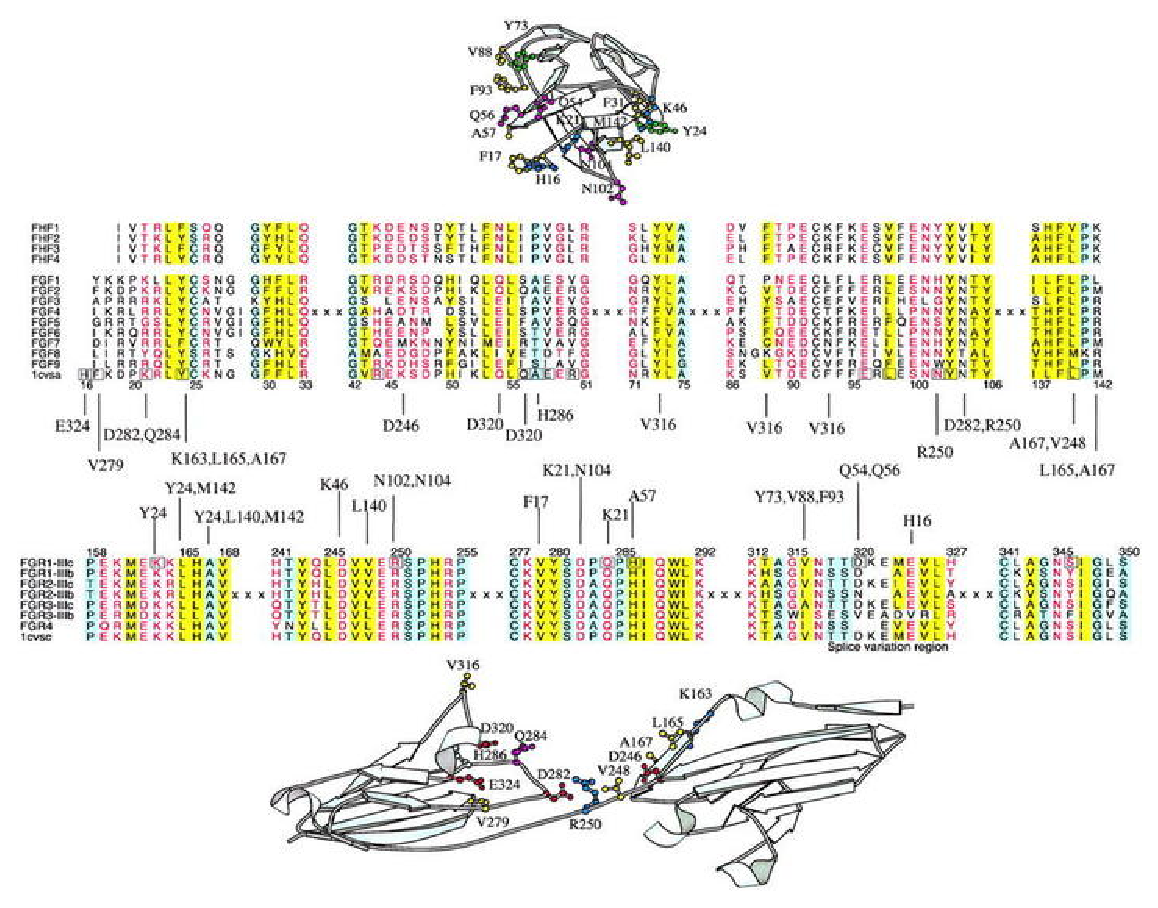
\includegraphics{prot2prot_interface}
\caption%[]
{
Interfaz entre dos prote\'\i{}nas que forman un heterod\'{i}mero y conservaci\'{o}n de secuencia de los que establecen contactos. 
Figura tomada de \citet{Aloy2002a}. Copyright (2002) National Academy of Sciences.
}
\label{fig:prot2protI}
\end{center}
\end{figure}

\begin{figure}
\begin{center} 
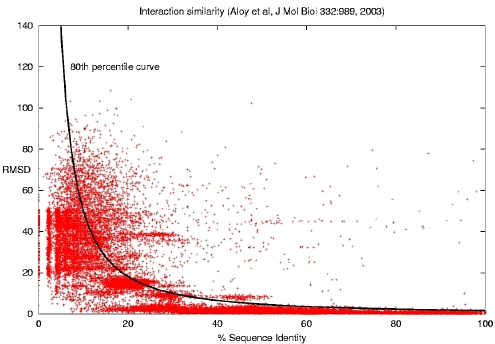
\includegraphics{simint}
\caption%[]
{
Relaci\'{o}n entre la conservaci\'{o}n de secuencia y estructura en las interfaces entre prote\'\i{}nas.
Figura tomada de \citet{Aloy2003} y reproducida con permiso de los autores.
}
\label{fig:prot2prot_cons}
\end{center}
\end{figure}
%\htmladdnormallink{http://www.russell.embl.de/simint}{http://www.russell.embl.de/simint}

\begin{figure}
%\htmlimage{scale=1.5}
\begin{center} 
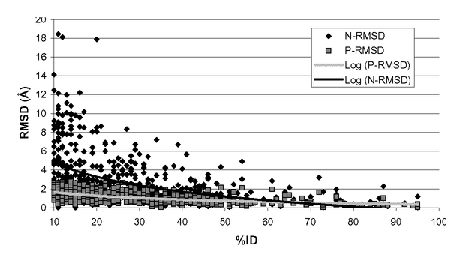
\includegraphics{protDNA_interface_cons}
\caption%[]
{
Relaci\'{o}n entre la conservaci\'{o}n de secuencia y estructura en las interfaces entre 
prote\'\i{}nas (P) y \'{a}cidos nucleicos (N). Figura tomada de \citet{ContrerasMoreira2006}
y reproducida con permiso de los autores.}.
\label{fig:prot2DNA_cons}
\end{center}
\end{figure}

Estas observaciones pueden resumirse en esta generalizaci\'{o}n: 
prote\'{i}nas con secuencias parecidas suelen tener interfaces similares cuando forman complejos. 
Los algoritmos que vamos a ver a continuaci\'{o}n, que se justifican (al menos en parte)
por estas observaciones, se han aplicado para el dise\~no de prote\'{i}nas y sus interfaces,
puesto que muchas de sus funciones conocidas dependen de interacciones con otras mol\'{e}culas.
Su diagrama de flujo gen\'{e}rico podr\'{i}a ser \'{e}ste:

\begin{figure}
%\htmlimage{scale=1.5}
\begin{center} 
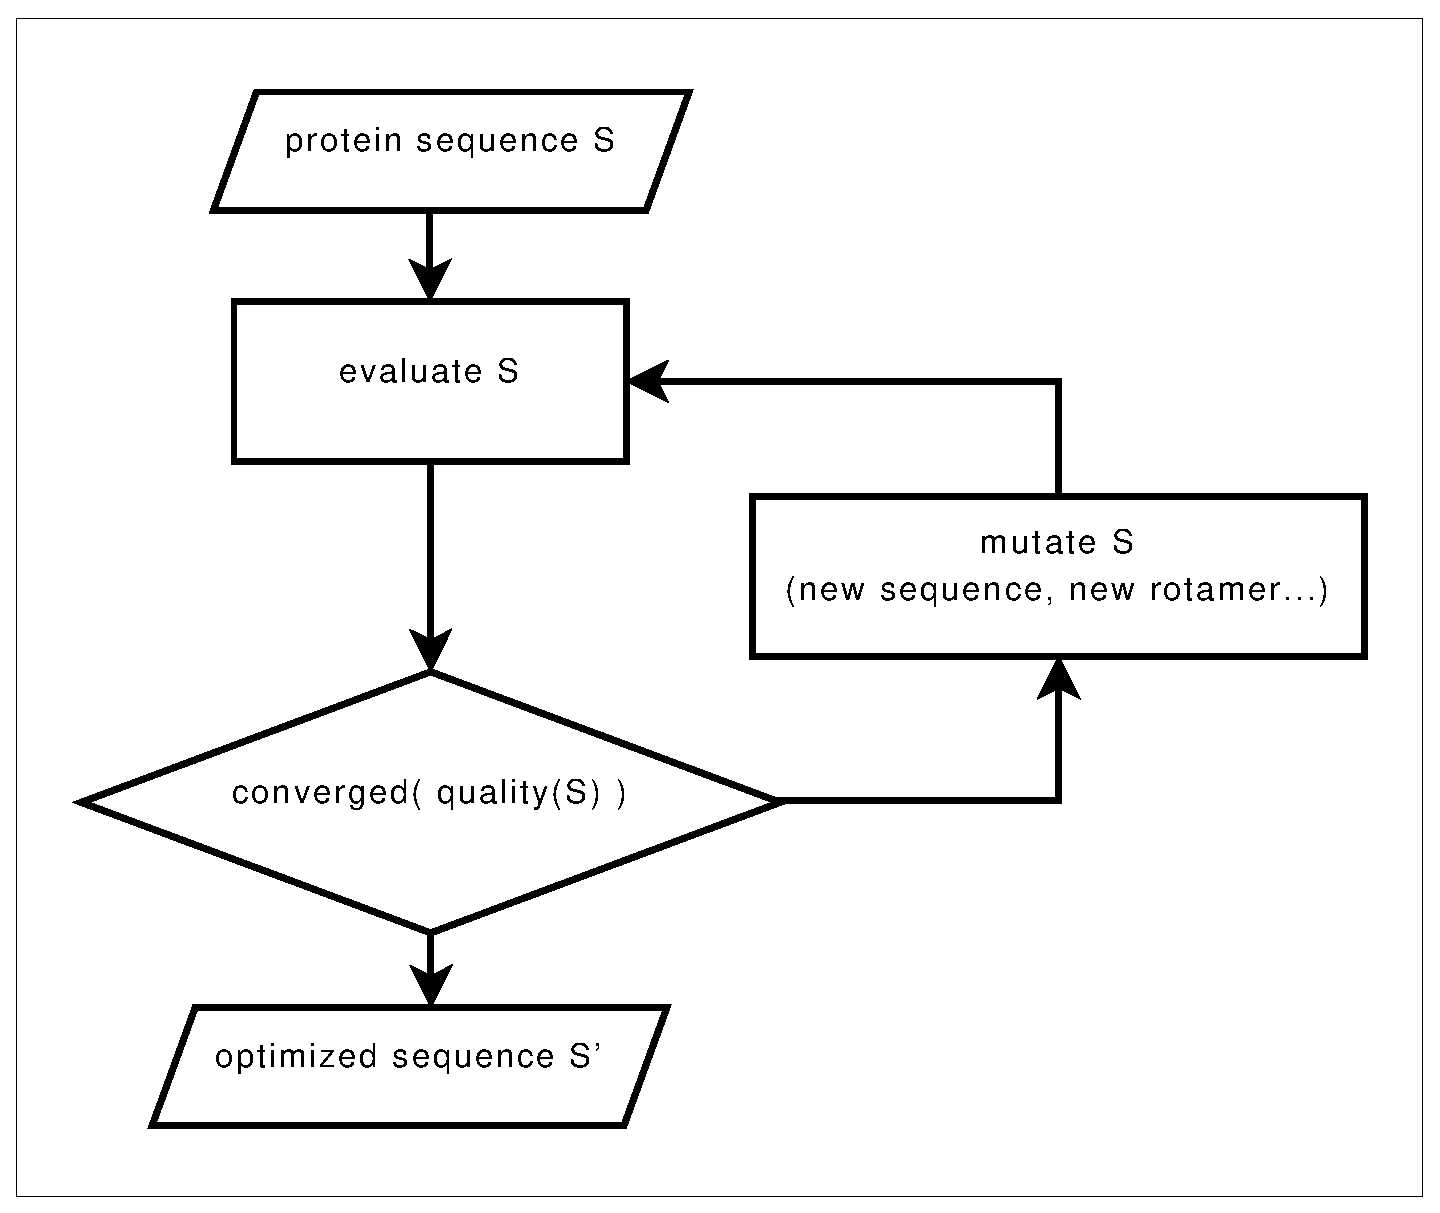
\includegraphics{design}
\caption%[]
{
Protocolo gen\'{e}rico de dise\~no de prote\'{i}nas.
}
\label{fig:design}
\end{center}
\end{figure}


De todas maneras hay que ser conscientes de que no deja de ser una simplificaci\'{o}n centrarse solamente en la interfaz, 
pues sabemos que a veces los cambios en zonas lejanas de la prote\'{i}na son m\'{a}s importantes para su funci\'{o}n biol\'{o}gica, 
por ejemplo entre factores de transcripci\'{o}n par\'{a}logos \citep{Hudson2016}.

\section{Optimizaci\'{o}n de cadenas laterales en interfaces} \label{scwrl}

En ocasiones podemos asumir que el esqueleto pept\'{i}dico de una prote\'{i}na %(en ingl\'{e}s \italics{backbone}) 
no va a variar mucho al cambiar su secuencia, en particular cuando la similitud global de secuencia es alta.
Si se cumple esta condici\'{o}n es posible tratar de optimizar una secuencia de amino\'{a}cidos con
el fin de modificar su estabilidad, su actividad enzim\'{a}tica o su especificidad. Por ejemplo, 
en este art\'\i{}culo de \citet{Reina2002}, %\htmladdnormallink{este art\'\i{}culo}{./papers/PDZdesign2002.pdf} 
los autores redise\~nan una prote\'\i{}na para cambiar su afinidad por un ligando. En este caso, el algoritmo de 
dise\~no se basa en sustituir(mutar) de manera exhaustiva ciertas posiciones de la secuencia, por medio de
una biblioteca de rot\'{a}meros, que son posteriormente evaluadas.
%En \'{e}ste trabajo, dada una funcion de evaluaci\'{o}n que tratamos de optimizar, el algoritmo


\begin{figure}
\begin{center} 
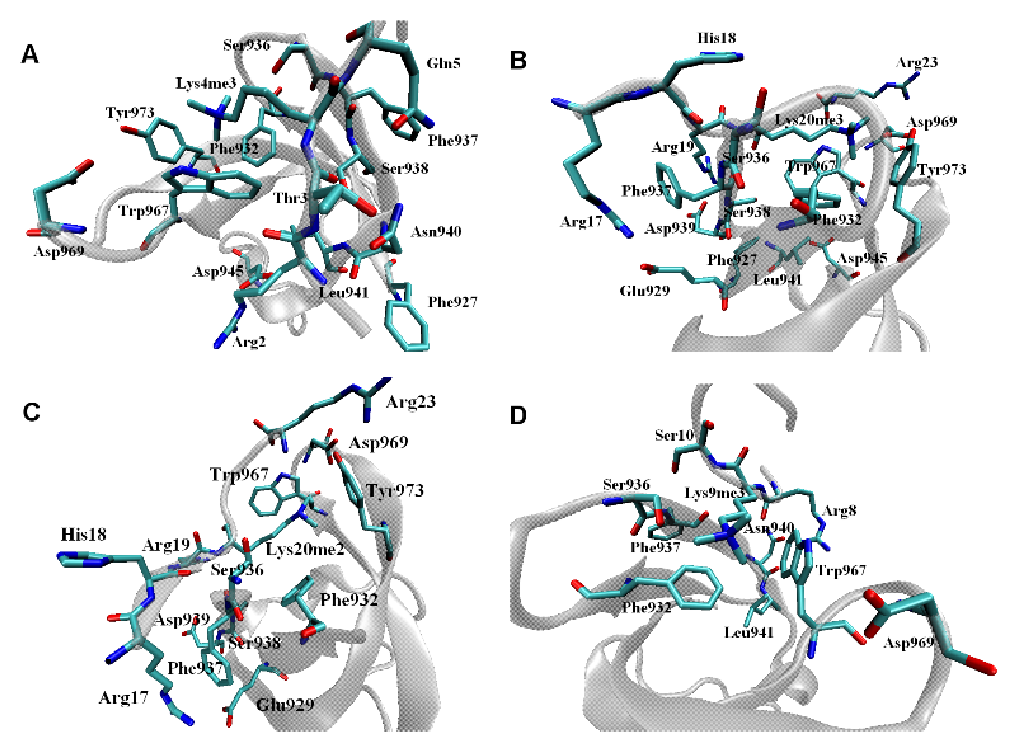
\includegraphics{JMJD2A-H3K3me3}
\caption%[]
{
Fotogramas de simulaciones de din\'{a}mica molecular (ver secci\'{o}n \ref{DM}) mostrando los rot\'{a}meros de residuos
de la histona demetilasa JMJD2A involucrados en el reconocimiento de p\'{e}ptidos H3K4me3 (A), H4K20me3 (B), H4K20me2 (C) y H3K9me3 (D).
Figura tomada de \citet{Ozboyaci2011} y reproducida con permiso de los autores.
}
\label{fig:JMJD2A}
\end{center}
\end{figure}

%\begin{figure}
%\begin{center} 
%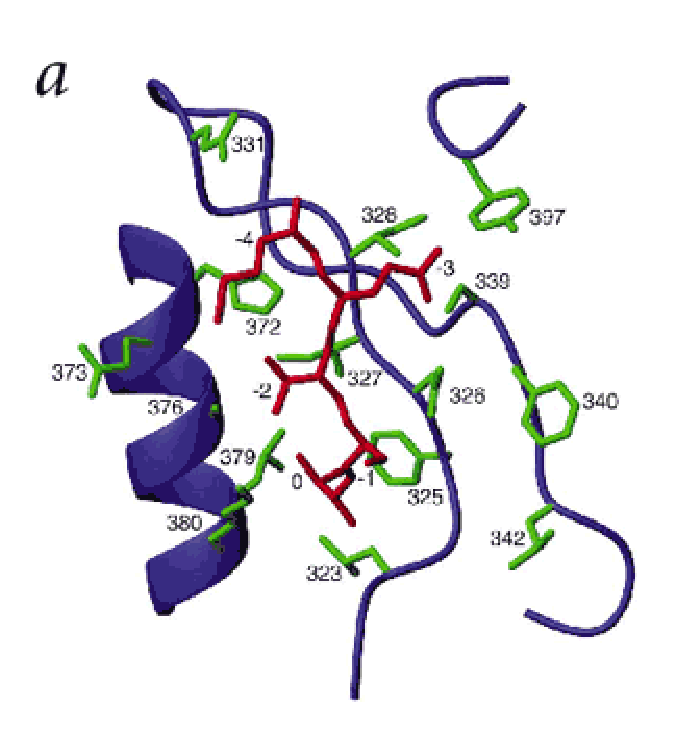
\includegraphics{PDZ}
%\caption%[]
%{
%Diagrama mostrando los rot\'{a}meros m\'{a}s importantes para el reconocimiento PDZ-p\'{e}ptido, tomado de \citet{Reina2002}.
%}
%\label{fig:PDZ}
%\end{center}
%\end{figure}

Para entender en mayor detalle este experimento podemos aprender a utilizar el programa 
\htmladdnormallink{SCWRL}{http://dunbrack.fccc.edu/scwrl4} \citep{Bower1997}   
(en ingl\'{e}s se pronuncia algo as\'\i{} como 'ardilla') 
que calcula las conformaciones de cadenas laterales (rot\'{a}meros) de una prote\'\i{}na dada la geometr\'{i}a 
local (en concreto los \'{a}ngulos $\phi$ y $\psi$) del esqueleto y las conformaciones de los residuos vecinos.
SCWRL explora una biblioteca de cadenas laterales precompiladas, extra\'\i{}das del Protein Data Bank.

\begin{itemize}

\item Identifica y descarga las estructuras PDB utilizadas en el art\'\i{}culo de \citet{Reina2002},
cu\'{a}l de ellas incluye las coordenadas de un p\'{e}ptido? Selecciona \'{e}sa.

\item Mediante SCWRL calcula los rot\'{a}meros m\'{a}s adecuados para el p\'{e}ptido y comp\'{a}ralos con
los de las coordenadas experimentales obtenidas del PDB. Observas diferencias importantes?

\item Con SCWRL muta el p\'{e}ptido ligando usando algunas de las secuencias del art\'\i{}culo (opci\'{o}n \verb+-s+).

\item Para cada p\'{e}ptido mutante calcula con SCWRL los rot\'{a}meros m\'{a}s
adecuados de los residuos del dominio \htmladdnormallink{PDZ}{http://pfam.xfam.org/family/PF00595} 
que lo reconoce. Ves qu\'{e} residuos han cambiado de rot\'{a}mero?

\end{itemize}

Puede parecer razonable asumir que la geometr\'{i}a del esqueleto de la prote\'\i{}na se ve poco afectada al sustituir de manera 
aleatoria rot\'{a}meros. Sin embargo, hay estudios que observan que al muestrear cadenas laterales de 
amino\'{a}cidos se producen peque\~nos cambios conformacionales locales, que se pueden reproducir 
usando el algoritmo de \italics{backrub} de \citet{Davis2006}.

%%%%%%%%%%%%%%%%%%%%%%%%%%%%%%%%%%%%%%%%%%%%%%%%%%%%%%%%%%%%%%%%%%%%%%%%

\section{Modelando nucle\'{o}tidos dentro de una doble h\'{e}lice de DNA} \label{modelnt}

Al igual que con SCWRL es posible explorar los rot\'{a}meros de ciertas posiciones de una estructura proteica (ver \ref{scwrl}), 
con el siguiente c\'{o}digo, parte del algoritmo DNAPROT de \citet{Espinosa2008}, 
podemos sustituir bases nitrogenadas a lo largo 
de una doble h\'{e}lice de DNA en formato PDB, importando el m\'{o}dulo \htmladdnormallink{bases}{./code/bases.py} y descargando
las coordenadas cristalogr\'{a}ficas de la prote\'{i}na dnaA (\htmladdnormallink{PDB 1J1V}{http://www.rcsb.org/pdb/explore.do?structureId=1j1v}):

\begin{figure}
\begin{center} 
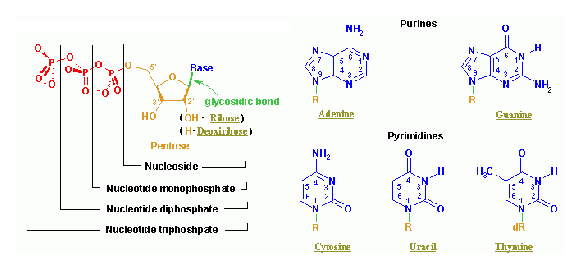
\includegraphics{nucleotides}
\caption%[]
{
Nomenclatura y numeraci\'{o}n de los nucle\'{o}tidos y sus \'{a}tomos, tal como se emplea en el formato PDB,
tomada de \htmladdnormallink{Wikipedia}{http://en.wikipedia.org/wiki/Nucleotide} y reproducida con permiso.
}
\label{fig:nucleotides}
\end{center}
\end{figure}

\verbatiminput{code/prog4.1.py}

Para este tipo de manipulaciones moleculares de \'{a}cidos nucleicos es muy recomendable el software 
\htmladdnormallink{3DNA}{http://x3dna.org}, que puedes descargar o usar desde una interfaz web \citep{Lu2008}.

%%%%%%%%%%%%%%%%%%%%%%%%%%%%%%%%%%%%%%%%%%%%%%%%%%%%%%%%%%%%%%%%%%%%%%%%

\section{Interacciones no covalentes: puentes de hidr\'{o}geno en la interfaz} \label{Hbonds}

El estudio experimental y te\'{o}rico de las interacciones entre prote\'{i}nas 
(\htmladdnormallink{\italics{protein-protein interactions}}{http://en.wikipedia.org/wiki/Protein-protein_interaction})
sembr\'{o} el inter\'{e}s por entender los mecanismos que explicaban la especificidad de su reconocimiento.
Obviamente \'{e}ste es un proceso termodin\'{a}mico complejo, donde se conjugan 
\htmladdnormallink{afinidades}{http://en.wikipedia.org/wiki/Chemical_affinity} y especificidades, pero en muchas ocasiones los 
protagonistas son los puentes de hidr\'{o}geno de la interfaz, que naturalmente dependen de la secuencia o estructura primaria, 
puesto que no todos los amino\'{a}cidos pueden actuar como donadores o aceptores \citep{Kortemme2003}.

\begin{figure}
\begin{center} 
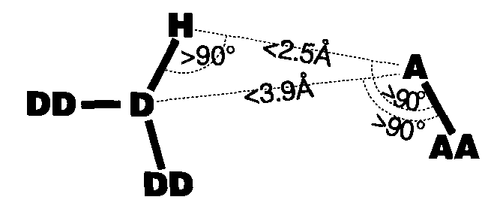
\includegraphics{Hbondgeo}
\caption%[]
{
Geometr\'{i}a ideal de un puente de hidr\'{o}geno, donde A es el grupo aceptor, D el donador,
AA es el grupo antecedente a A y H es el hidr\'{o}geno.
Figura de \citet{McDonald1994} reproducida con permiso de los autores.
}
\label{fig:Hbondgeo}
\end{center}
\end{figure}

En las secciones anteriores hemos probado algoritmos para muestrear, por un lado, rot\'{a}meros de cadenas laterales 
de amino\'{a}cidos y, por otro, bases nitrogenadas de nucle\'{o}tidos, bajo la misma premisa de que la geometr\'{i}a 
del esqueleto pept\'{i}dico y de la doble h\'{e}lice de DNA va a variar muy poco al sustituir un n\'{u}mero peque\~no 
de cadenas laterales y bases nitrogenadas. En esta secci\'{o}n vamos un paso m\'{a}s all\'{a}, puesto 
que adem\'{a}s de muestrear es necesario evaluar la especificidad del reconocimiento de las interfaces modeladas, 
por ejemplo estimando la formaci\'{o}n de puentes de hidr\'{o}geno.

\begin{figure}
\begin{center} 
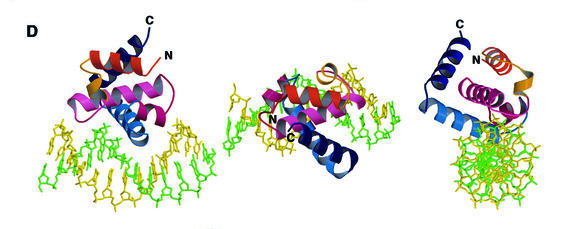
\includegraphics{dnaA}
\caption%[]
{
La prote\'{i}na \htmladdnormallink{dnaA}{http://floresta.eead.csic.es/3dpwm/complexes/1j1v_A.html} en complejo 
con ADN. Figura tomada de \cite{Fujikawa2003}. Copyright (2003) Nucleic Acids Research.
}
\label{fig:dnaA}
\end{center}
\end{figure} %https://www.ncbi.nlm.nih.gov/pmc/articles/PMC153737/

El punto de partida para presentar este algoritmo es la estructura del complejo de dnaA y su sitio operador, tras a\~nadir con
\htmladdnormallink{Open Babel}{http://openbabel.org/wiki/Main_Page} los \'{a}tomos de hidr\'{o}geno que puedan faltar de un fichero
en formato PDB (ver \htmladdnormallink{\italics{script}}{./code/add_hydrogens.py}).
Por ejemplo, partiendo del complejo capturado en el archivo \htmladdnormallink{PDB 1J1V}{http://www.rcsb.org/pdb/explore.do?structureId=1j1v}, 
que ya usamos en el apartado \ref{modelnt}, obtenemos \htmladdnormallink{1j1v\_withH.pdb}{./files/1j1v_withH.pdb}. 
Una vez realizado este paso preliminar,
por medio del siguiente c\'{o}digo podemos identificar los puentes de la interfaz prote\'{i}na-DNA, como har\'{i}amos con el programa
\htmladdnormallink{HBPLUS}{http://www.ebi.ac.uk/thornton-srv/software/HBPLUS} \citep{McDonald1994}:
\verbatiminput{code/prog4.2.py}

%%%%%%%%%%%%%%%%%%%%%%%%%%%%%%%%%%%%%%%%%%%%%%%%%%%%%%%%%%%%%%%%%%%%%%%%%%%%%%%%%%%%%%%%

\section{Interfaces entre prote\'{i}na, DNA y RNA: endonucleasas CRISPR-Cas guiadas por RNA} \label{CRISPR}

A veces no necesitamos modelar una interfaz molecular, pero s\'{i} comprenderla, para dise\~{n}ar experimentos.
Esto ocurre con las endonucleasas \htmladdnormallink{CRISPR-Cas}{http://wwwuser.cnb.csic.es/~montoliu/CRISPR}, 
herramientas de edici\'{o}n gen\'{o}mica en principio 
m\'{a}s sencillas de emplear que las prote\'{i}nas TALEN o las endonucleasas fusionadas con dominios Zinc Finger (ZFN).

\begin{figure}
\begin{center} 
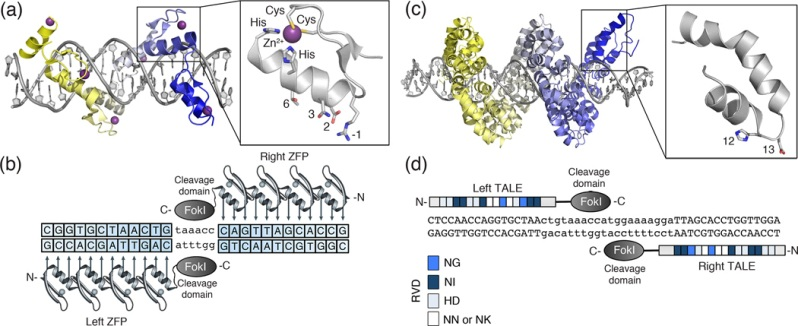
\includegraphics{ZFNTALEN}
\caption%[]
{
Dominios Zinc Finger (ZF, izq) y transcription activator-like effector (TALEN, dcha) fusionados con endonucleasas FokI.
En ambos casos se muestran en cajas los nucleotidos reconocidos por cada dominio. 
Mientras cada ZF reconoce en general 3 bases, cada TALEN reconoce solamente una.
Figura de \cite{Gaj2013} reproducida con permiso.
}
\label{fig:ZFNTALEN}
\end{center}
\end{figure}

Estos sistemas se han usado, por ejemplo, para inducir mutaciones heredables en loci seleccionados de plantas, incluso en especies poliploides
como el trigo panadero \citep{Wang2014,Lawrenson2015}. 
Para ello es preciso hacer an\'{a}lisis de secuencias con el fin de elegir las secuencias adecuadas, 
normalmente \'{u}nicas en el genoma. 
En el caso de las endonucleasas Cas \citep{Stella2017}, polip\'{e}ptidos de m\'{a}s de 1000 amino\'{a}cidos,
las secuencias diana deben elegirse respetando la arquitectura 
de la interfaz entre prote\'{i}na, DNA y RNA, que requiere un motivo de entre 3 y 5b adyacente a la diana,
llamado PAM (\italics{protospacer adjacent motif}). Adem\'{a}s de la estructura de estos complejos, 
normalmente es necesario determinar experimentalmente \italics{in vitro} e \italics{in vivo} la 
tasa de cortes no deseados o qu\'{e} partes del RNA gu\'{i}a (sgRNA) m\'{a}s sensibles en la hibridaci\'{o}n \citep{Cisse2012,Zheng2017}.
Se han empleado asimismo modelos de din\'{a}mica molecular para estudiar la mec\'{a}nica de estos complejos \citep{Zheng2017w}.

\begin{figure}
\begin{center} 
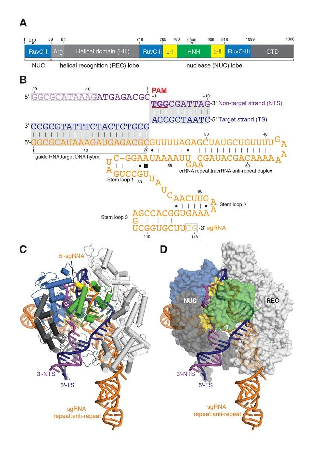
\includegraphics{Cas9}
\caption%[]
{
Estructura del complejo Cas9-sgRNA-dsDNA.
A) Dominios de Cas9 de Streptococcus pyogenes. 
B) Esquema del complejo sgRNA-DNAdiana. La hebra DNA diana se muestra en azul oscuro, la secuencia PAM se subraya, y sgRNA se muestra en naranja. 
Los sitios de corte no se muestran, ver \citet{Stella2017}.
C,D) Estructuras del complejo ternario.
Figura de \cite{Jiang2016} reproducida con permiso.
}
\label{fig:Cas}
\end{center}
\end{figure}

%\begin{figure}
%\begin{center} 
%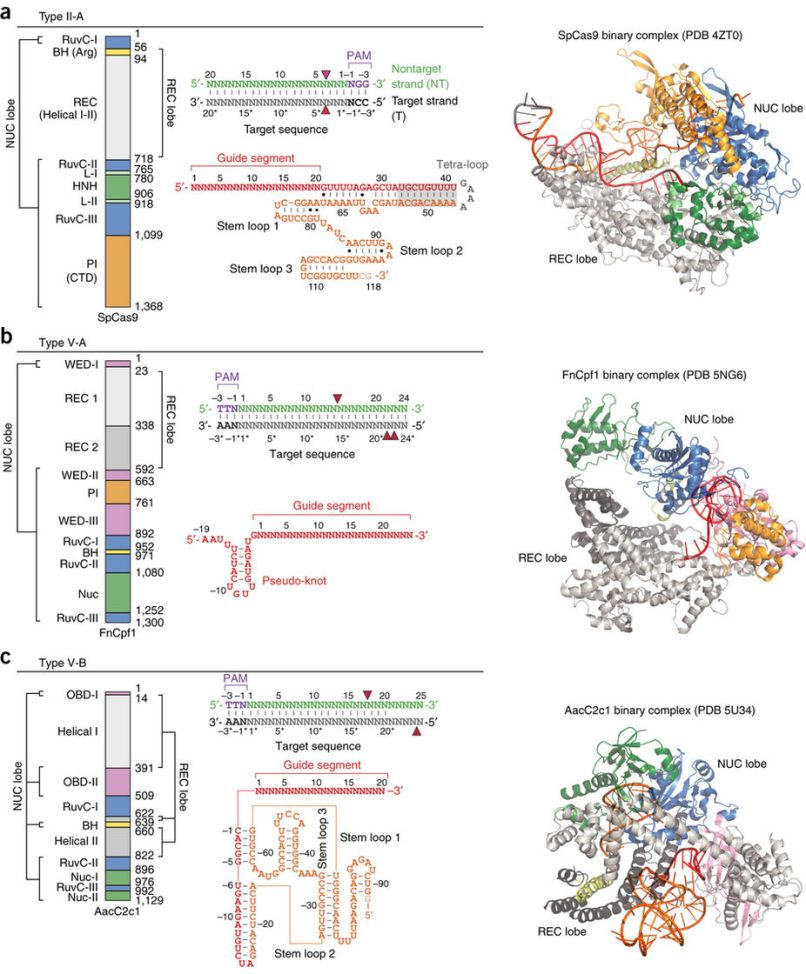
\includegraphics{Cas3D}
%\caption%[]
%{
%Composici\'{o}n de dominios de enzimas Cas de tipo II-A (Cas9), V-A (Cpf1) y V-B (C2c1) en complejo con crRNAs.
%Se muestran los segmentos gu\'{i}a, de 20b, adyacentes a motivos PAM, y los puntos de corte en cada
%hebra. Figura de \citep{Stella2017}.
%}
%\label{fig:Cas}
%\end{center}
%\end{figure}


%%%%%%%%%%%%%%%%%%%%%%%%%%%%%%%%%%%%%%%%%%%%%%%%%%%%%%%%%%%%%%%%%%%%%%%%%%%%%%%%%%%%%%%%

\section{Modelando interfaces moleculares por homolog\'{i}a} \label{dockhom}

Podemos aprovechar las observaciones de las figuras \ref{fig:prot2prot_cons} y \ref{fig:prot2DNA_cons} 
para estudiar u optimizar una interfaz molecular en base a la estructura de otras mol\'{e}culas similares.

Hay muchas herramientas disponibles para modelar interfaces entre prote\'{i}nas,
desde herramientas sencillas como 
\htmladdnormallink{InterPreTS}{http://www.russelllab.org/cgi-bin/tools/interprets.pl} o
\htmladdnormallink{PPI3D}{http://bioinformatics.ibt.lt/ppi3d},
que no cambian la geometr\'{i}a de la estructura molde usada como punto de apoyo,
a protocolos m\'{a}s complejos que ajustan el acoplamiento por \italics{docking},
como \htmladdnormallink{PRISM}{http://cosbi.ku.edu.tr/prism}.
Hay tambi\'{e}n herramientas especializadas en el estudio de interfaces en el contexto
de enfermedades asociadas a mutaciones (\htmladdnormallink{InteractomeINSIDER}{http://interactomeinsider.yulab.org})
o en el dise\~{n}o de anticuerpos \citep{Lapidoth2015,Baran2017}.

En este apartado combinamos algunas de las herramientas empleadas en otras secciones para estudiar, por ejemplo, tres diferentes 
\htmladdnormallink{factores sigma70}{http://en.wikipedia.org/wiki/Sigma_factor} 
de la bacteria \italics{Rhizobium etli CFN42}, 
como son \htmladdnormallink{SigA}{http://www.uniprot.org/uniprot/Q2K619},
\htmladdnormallink{rpoH1}{http://www.uniprot.org/uniprot/Q2K4Y1} y
\htmladdnormallink{rpoH2}{http://www.uniprot.org/uniprot/Q2K316}.
De ninguna de ellas conocemos actualmente su estructura en complejo con ADN,
pero s\'{i} sabemos que SigA reconoce con cierta especificidad el consenso CTTGACN[16-23]TATNNT, 
como se explica en detalle en este trabajo de \cite{RamirezRomero2006}, 
donde entre otras cosas tambi\'{e}n estiman la estabilidad
de las regiones promotoras, como vimos en la secci\'{o}n \ref{dna1}.

Para seleccionar estructuras molde que nos sirvan para construir modelos podemos,
como vimos en la secci\'{o}n \ref{CM}, buscar directamente en el \htmladdnormallink{PDB}{http://www.rcsb.org/pdb}.
Sin embargo, en este caso iremos m\'{a}s r\'{a}pido si consultamos el repositorio 
\htmladdnormallink{3D-footprint}{http://floresta.eead.csic.es/3dfootprint} \citep{ContrerasMoreira2010}, 
que contiene solamente el conjunto actualizado de complejos prote\'{i}na-DNA.
Si pegamos en el motor de b\'{u}squeda de 3D-footprint las secuencias de estas 3 prote\'{i}nas
nos encontramos con que el complejo 
\htmladdnormallink{1rio\_H}{http://floresta.eead.csic.es/3dfootprint/complexes/1rio_H.html}
parece ser el mejor molde en todos los casos, ya que 
\htmladdnormallink{3iyd\_F}{http://floresta.eead.csic.es/3dfootprint/complexes/3iyd_F.html}
es un complejo resuelto por microscop\'{i}a con muy poca resoluci\'{o}n:



Asimismo podemos observar que el logo de \htmladdnormallink{1rio\_H}{http://floresta.eead.csic.es/3dfootprint/complexes/1rio_H.html}
se corresponde bastante bien con la caja -35 descrita en el art\'{i}culo de \cite{RamirezRomero2006}:
\begin{center} 
\texttt{cTTGACT}\\
\texttt{||||||+}\\
\texttt{CTTGACN}\\
\end{center} 
lo cual no es sorprendente dado que SigA tiene un conjunto de residuos de interfaz, aquellos que contactan con las bases nitrogenadas,
conservado respecto al de \htmladdnormallink{1rio\_H}{http://floresta.eead.csic.es/3dfootprint/complexes/1rio_H.html}. Sin embargo, no 
ocurre lo mismo con rpoH1 y rpoH2, que presentan mutaciones en la interfaz.

El ejercicio de esta secci\'{o}n consiste en:
\begin{itemize}

\item Construir modelos por homolog\'{i}a de 
\htmladdnormallink{rpoH1}{http://www.uniprot.org/uniprot/Q2K4Y1} y
\htmladdnormallink{rpoH2}{http://www.uniprot.org/uniprot/Q2K316}, en presencia de la mol\'{e}cula de ADN de 
\htmladdnormallink{1rio\_H}{http://floresta.eead.csic.es/3dfootprint/complexes/1rio_H.html}. Puedes probar MODELLER, 
como avanzamos en la secci\'{o}n \ref{CM}, siguiendo el 
\htmladdnormallink{tutorial avanzado}{http://salilab.org/modeller/tutorial/advanced.html}, que contiene una parte sobre 
\italics{Modeling ligands in the binding site}, la herramienta web 
\htmladdnormallink{TFmodeller}{http://www.ccg.unam.mx/tfmodeller/}, o cualquier m\'{e}todo que se te ocurra, 
pero es esencial que el modelo contenga las coordenadas de ADN del molde.

\item Escribir un programa, que puede aprovechar c\'{o}digo de otras secciones de este curso, para analizar las interfaces
moleculares de los modelos rpoH1 y rpoH2, con el fin de elucidar si se conservan las interacciones no covalentes
de reconocimiento de bases nitrogenadas.

\item Si cambiase alguna de las interacciones, qu\'{e} posiciones del consenso de 
\htmladdnormallink{1rio\_H}{http://floresta.eead.csic.es/3dfootprint/complexes/1rio_H.html}
esperas que cambien?

\end{itemize}




%%%%%%%%%%%%%%%%%%%%%%%%%%%%%%%%%%%%%%%%%%%%%%%%%%%%%%%%%%%%%%%%%%%%%%%%

\section{Modelando interfaces moleculares mediante docking}

En la secci\'{o}n \ref{dockhom} aprovech\'{a}bamos las coordenadas de un complejo molecular conocido
para aproximar la interfaz de una secuencia hom\'{o}loga. Cuando no disponemos de estructuras 
de referencia, el estudio de las conformaciones que adoptan las macromol\'{e}culas cuando interaccionan 
de forma transitoria es aun m\'{a}s dif\'{i}cil, con costes computacionales poco asumibles.
La raz\'{o}n de esto es que hay muchos grados de libertad y un gran n\'{u}mero de \'{a}tomos del sistema pueden moverse. 
%En un experimento de \italics{docking} las mol\'{e}culas pueden ser flexibles y en general son protagonistas las 
%interacciones no covalentes, como los puentes de hidr\'{o}geno (ver secciones \ref{macro1:intnocov} y \ref{Hbonds}).
Por tanto, los algoritmos de \htmladdnormallink{\italics{docking}}{http://en.wikipedia.org/wiki/Macromolecular_docking} 
suelen emplear estrategias para ahorrar recursos, como por ejemplo el uso de transformadas de Fourier en vez del empleo 
expl\'{i}cito de matrices de rotaci\'{o}n y traslaci\'{o}n \citep{Katchalski1992}.

Un subproblema espec\'{i}fico es el acoplamiento entre una enzima y su sustrato, una tarea para la que la informaci\'{o}n
gen\'{o}mica (operones) puede ser muy valiosa \citep{Zhao2013}.

Adem\'{a}s de bancos de pruebas publicados por algunos desarrolladores \citep{Yu2016}, 
desde el a\~no 2001 hay en marcha un experimento colectivo (\htmladdnormallink{CAPRI}{http://www.ebi.ac.uk/msd-srv/capri}) 
donde regularmente se ponen a prueba los diferentes algoritmos existentes
para predecir, antes de su publicaci\'{o}n, las poses de complejos proteicos cuyas estructuras se han resuelto experimentalmente 
(normalmente por cristalograf\'{i}a).  

%La \htmladdnormallink{lista de programas}{http://www.imb-jena.de/~rake/Bioinformatics_WEB/dd_tools.html} 
La lista de programas de acoplamiento molecular o \italics{docking} es muy amplia, por lo que puede ser buena idea consultar los resultados recientes de CAPRI para seleccionar el software adecuado 
para nuestras necesidades. Un problema a\~nadido es que en mi experiencia \'{e}stos son programas 
hechos por definici\'{o}n para usuarios avanzados, que requieren de cierta experiencia sobre todo a la hora de interpretar los resultados.

\begin{figure}
\begin{center} 
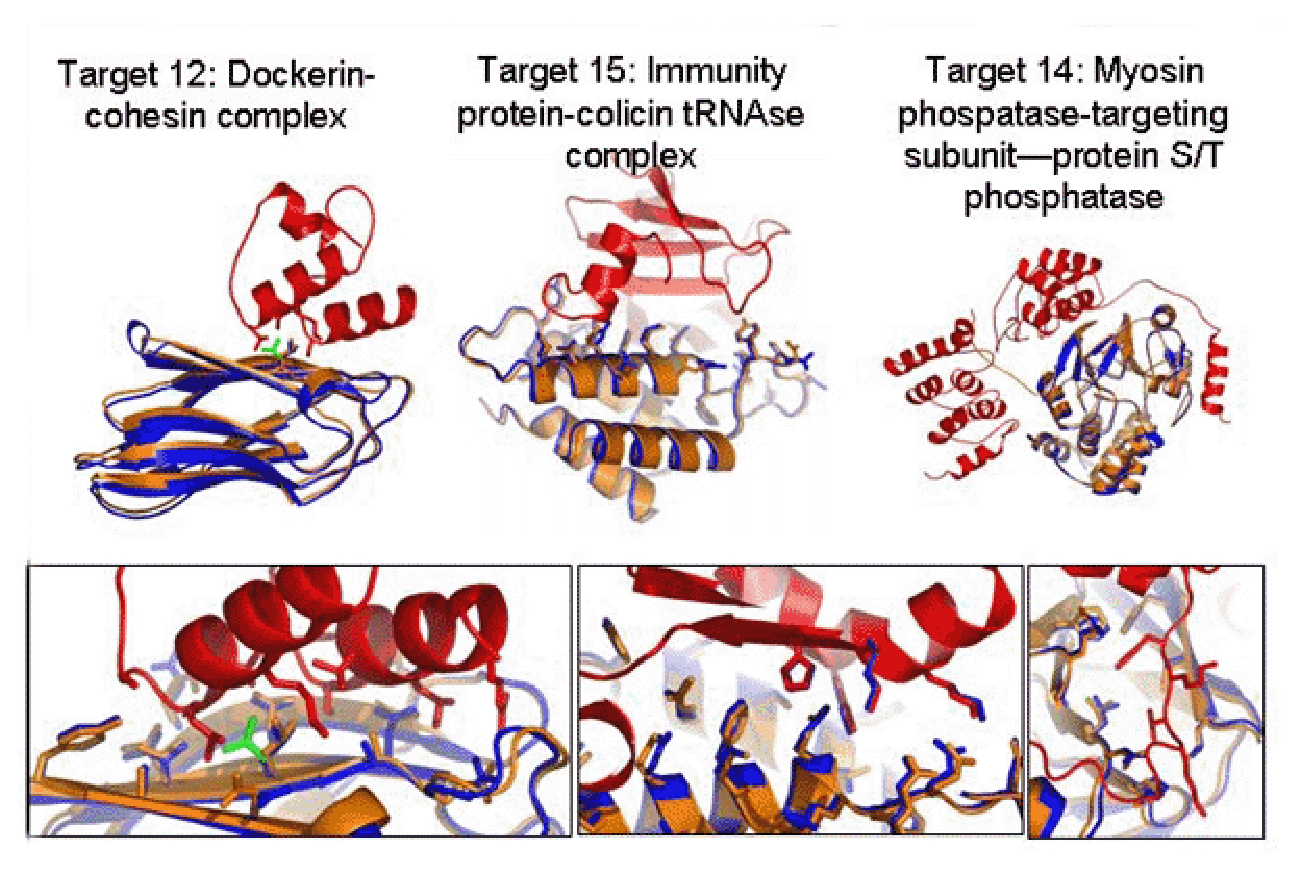
\includegraphics{docking3}
\caption%[]
{
Algunas predicciones de d\'{i}meros en CAPRI. 
Se muestran superposiciones de complejos predichos (azul) y resueltos experimentalmente por rayos X (rojo y naranja). 
En verde se destaca una cadena lateral que se reorienta al formarse el complejo. 
Figura tomada de \htmladdnormallink{https://boinc.bakerlab.org}{https://boinc.bakerlab.org/rosetta/rah/rah_docking.php}. 
}
\label{fig:docking}
\end{center}
\end{figure} 

%\begin{figure}
%\begin{center} 
%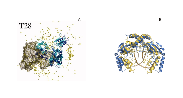
\includegraphics{docking2}
%\caption%[]
%{
%A: Problema de docking de \htmladdnormallink{CAPRI}{http://www.ebi.ac.uk/msd-srv/capri/},
%mostrando las coordenadas del ligando en estado libre (azul oscuro) superpuestas con las coordenadas finales (azul claro).
%B: Ejemplo de docking entre prote\'{i}nas y DNA con el algoritmo 
%\htmladdnormallink{HADDOCK}{http://www.nmr.chem.uu.nl/Software/haddock} \citep{vanDijk2006}.
%}
%\label{fig:docking}
%\end{center}
%\end{figure} 

Una buena manera de empezar a jugar con software de \italics{docking} puede ser instalando el software 
\htmladdnormallink{PyRosetta}{http://pyrosetta.org} \citep{Chaudhury2010}. Este software nos permite hacer,
de forma program\'{a}tica, una simulaci\'{o}n \italics{docking} en miniatura, en este caso entre un d\'{u}plex de ADN y 
el factor de transcripci\'{o}n DnaA , algo que puede plantearse simult\'{a}neamente como un problema cl\'{a}sico 
de \italics{docking} y como un problema de especificidad de reconocimiento:
\verbatiminput{code/prog4.3.py}

Como resultado de las simulaciones de \italics{docking} tendremos una serie de complejos, que pueden o no
mostrar interfaces relevantes en t\'{e}rminos biol\'{o}gicos, dependiendo de la profundidad del muestreo realizado
y el an\'{a}lisis posterior de los resultados, que obviamente requiere de cierta experiencia y sobre todo conocimiento
de las mol\'{e}culas implicadas. 
En concreto en el ejemplo 4.3, posiblemente como consecuencia del limitado muestreo (N=10), ninguna de las 
interfaces resultantes de mis simulaciones \htmladdnormallink{docking\_output.tgz}{./files/docking_output.tgz} consigue
reconstruir la interfaz descrita experimentalmente:

\begin{figure}
\begin{center} 
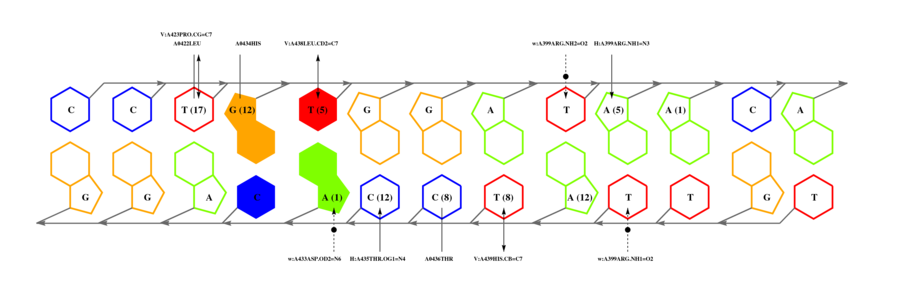
\includegraphics{1j1v_A_interface_thumb}
\caption%[]
{
Esquema del reconocimiento espec\'{i}fico de ADN en la interfaz de DnaA 
(\htmladdnormallink{PDB 1J1V}{http://www.rcsb.org/pdb/explore.do?structureId=1j1v}), tomado del repositorio
\htmladdnormallink{3D-footprint}{http://floresta.eead.csic.es/3dfootprint/complexes/1j1v_A.html}.
}
\label{fig:dnaA_intf}
\end{center}
\end{figure}

%Otra manera de analizar esta interfaz (o cualquier otra), si nos centramos en la especificidad de reconocimiento, podemos realizarla
%si enviamos sus coordenadas PDB al servidor 
%\htmladdnormallink{3D-footprint}{http://floresta.eead.csic.es/3dfootprint} \citep{ContrerasMoreira2010}. Por ejemplo, con el archivo
%\htmladdnormallink{1j1v\_withH.pdb}{./files/1j1v_withH.pdb} obtenemos:
%
%\begin{figure}
%\begin{center} 
%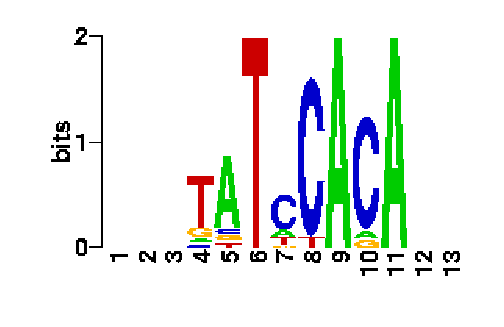
\includegraphics{1j1v_withH_logo}
%\caption%[]
%{
%Logo de las secuencias reconocidas por el factor de transcripcion dnaA, tal como lo calcula 
%\htmladdnormallink{3D-footprint}{http://floresta.eead.csic.es/3dfootprint/footprint.html} con las coordenadas
%de \htmladdnormallink{1j1v\_withH.pdb}{./files/1j1v_withH.pdb}.
%}
%\label{fig:footprint_logo}
%\end{center}
%\end{figure}

